\section{Detectare bandă}
\subsection*{Noțiuni introductive}
O primă componentă a aplicației de față este ceea care se ocupă de detecția benzii curente de circulație. Scopul acesteia este de a identifica marcajele, atât cele continue, cât și cele discontinue, însă fără a face o diferență concretă între ele, iar pe baza acestora indică banda curentă de circulație a mașinii.

\subsection*{Algoritm detecție bandă}
\subsubsection*{Etapa 1: Extragere regiune interes}

Această etapă are rolul de a elimina din imagine zonele redundante detecției \hyperlink{WaymoSystem}{[11]}. Atât în situația de față, cât și ulterior în cazul detecției de mașini, ne putem focusa pe o anumită zonă din cadrul frame-ului pentru a detecta banda curentă de circulație și ulterior mașina de pe aceasta. 
Această zonă este direct determinată de cameră, rezoluția acesteia, amplasarea camerei pe mașină, iar în funcție de toți acești factori se va crea un fișier de configurație specific montajului respectiv cu parametri necesari extragerii zonei de interes.

În figura 3.1 putem observa un exemplu concret.
\begin{figure}[!h]
	\centering
	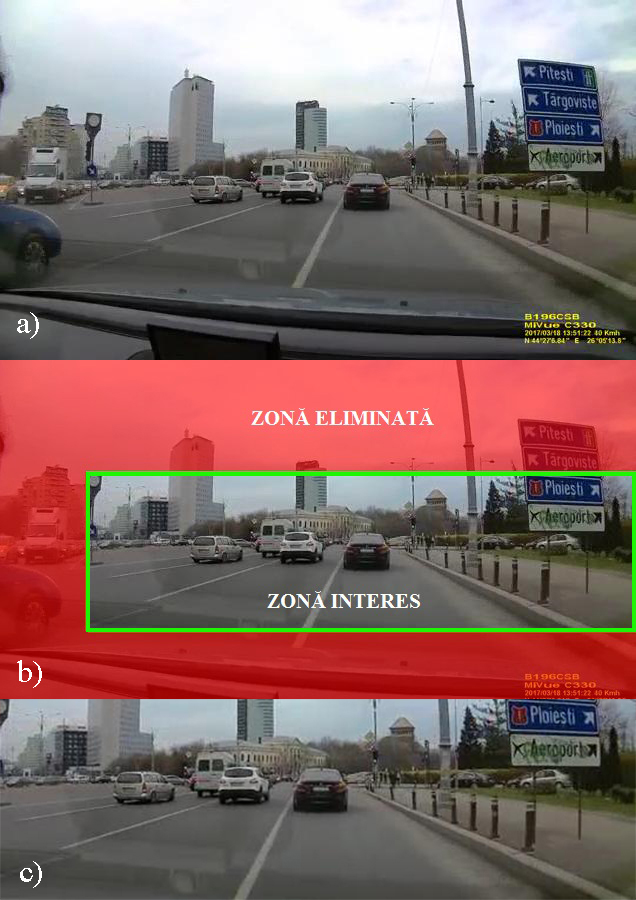
\includegraphics[max width=15cm,max height=15cm,keepaspectratio]{img_3_1}
	\caption[Zonă interes imagine]{a) Imaginea inițială b) Separația zonei de interes față de cea redundantă c) Imaginea de interes rezultată.}
\end{figure}

\subsubsection*{Etapa 2: Obținere imagine IPM}

Următoare etapă în procesul de detecție a benzii curente de circulație este cea în care schimba perspectiva de vizualizare a zonei de interes. Prin intermediul unui fișier de configurare se vor da parametri ce vor fi folosiți ulterior în funcția de obținere IPM. Fie A, B, C și D punctele extreme ale imaginii. Redefinim punctele B și C conform figurii 3.2. Cei doi vectori de puncte îi pasăm funcției $cv.getPerspectiveTransform$ din biblioteca OpenCV spre a obține matrice $M$ de trecere din perspectiva a), conform figurii 3.2, în perspectiva b). Matricea $M$ este folosită în continuare cu funcția $cv.warpPerspective$ pentru pentru a obține imaginea în planul IPM.
\begin{figure}[!h]
	\centering
	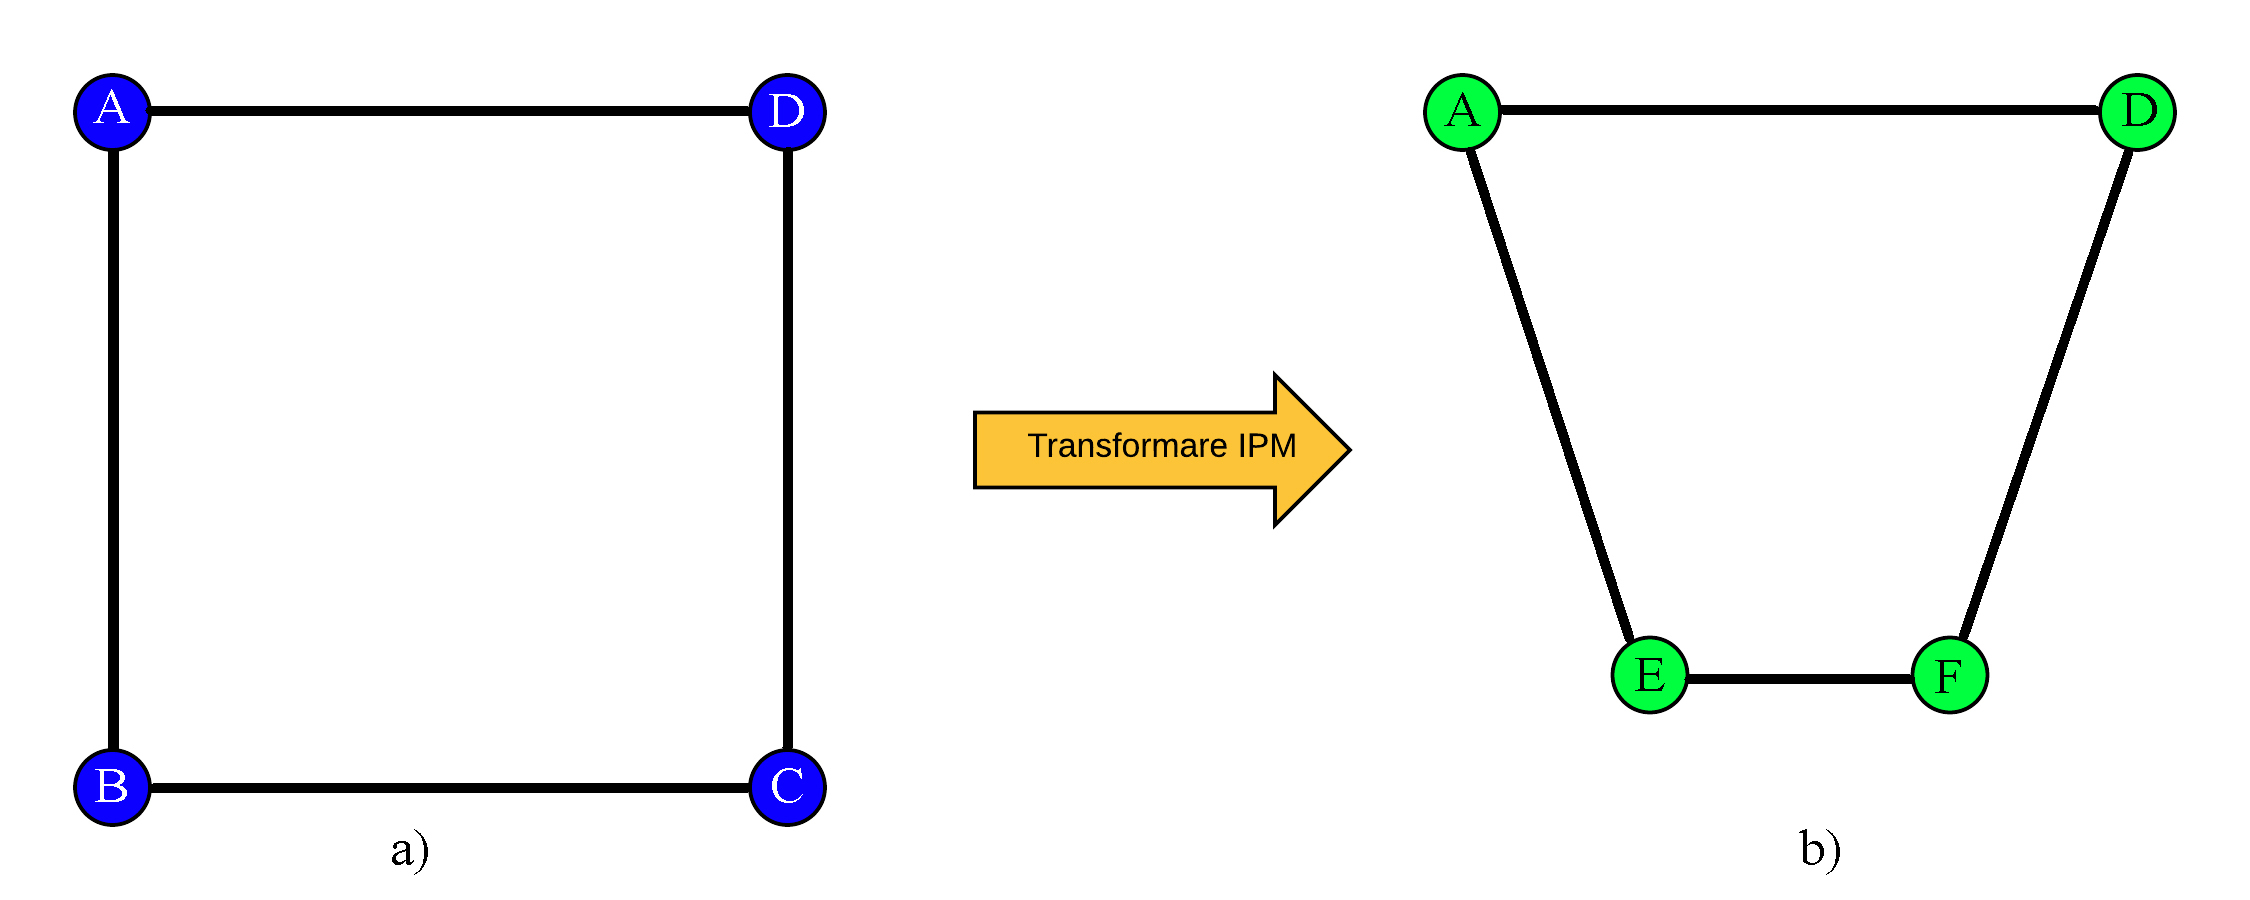
\includegraphics[max width=15cm,max height=15cm,keepaspectratio]{img_3_2}
	\caption[Transformare IPM]{a) Cadrul imaginii inițiale b) Cadrul imaginii IPM. Punctele B și C, din cadrul imaginii inițiale, sunt redefinite în punctele E și F.}
\end{figure}

În figura 3.3 este prezentat un exemplu practic.
\begin{figure}[!h]
	\centering
	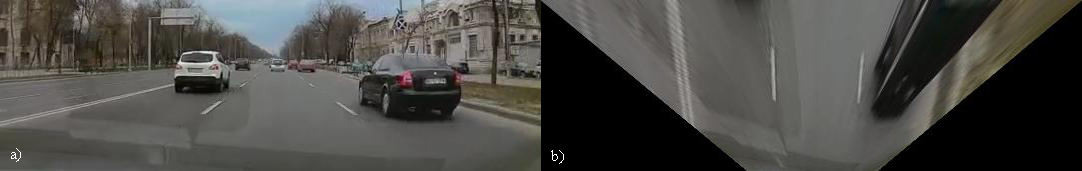
\includegraphics[max width=15cm,max height=15cm,keepaspectratio]{img_3_3}
	\caption[Transformare IPM în practică]{a) Imagine zonă interes b) Imaginea IPM asociată zonei de interes.}
\end{figure}


\subsubsection*{Etapa 3: Filtrarea imaginii IPM}

Filtrarea imaginii IPM are rolul de a păstra în imagine doar zonele cele mai plauzibile de a fi marcaje delimitatorii de bandă și eliminarea conținut nerelevant obiectivului nostru. Noua imagine va fi o imagine binară (alb - negru). Pentru filtrare se folosește filtrul Gaussian 2D orizontal dat de formula

\begin{align}
	d_x \xor (h \xor I) = (d_x \xor h) \xor I
\end{align}
\begin{align}
	d_y \xor (h \xor I) = (d_y \xor h) \xor I
\end{align}

unde

$d_x$, $d_y$ - reprezintă filtrele de derivare;

$h$ - reprezintă filtrul Gaussian;

$I$ - reprezintă imaginea.

După aplicarea acestui filtru, matricea rezultată va mai fi filtrată cu un prag, astfel toate valorile din matrice se se află sub acel prag vor deveni 0 celelalte păstrându-și intensitatea neschimbată \hyperlink{WaymoSystem}{[11]}.

În figura 3.4 putem vedea o astfel de imagine IPM filtrată.
\begin{figure}[!h]
	\centering
	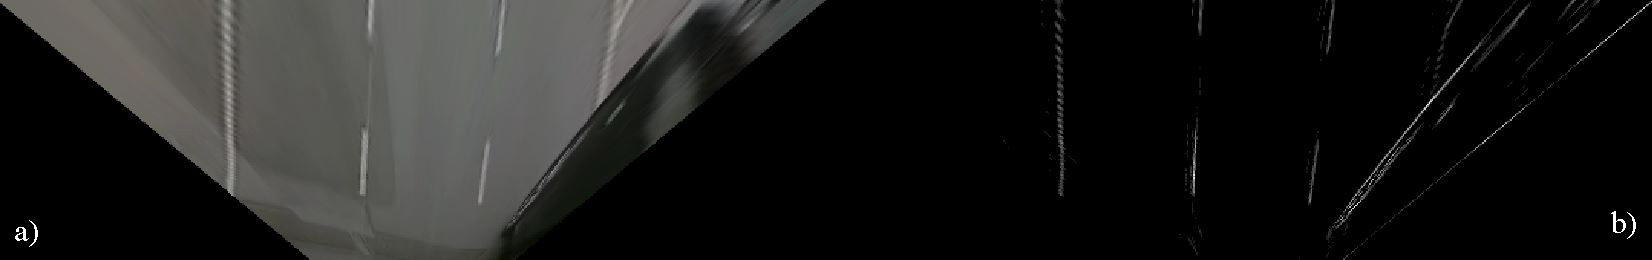
\includegraphics[max width=15cm,max height=15cm,keepaspectratio]{img_3_4}
	\caption[Imagine IPM filtrată]{a) Imaginea IPM b) Imaginea IPM filtrată.}
\end{figure}

\subsubsection*{Etapa 4: Extragere linii din imaginea filtrată}

În continuare ne ocupăm de extragerea potențialelor linii din imaginea filtrată. Pentru aceasta realizăm în primă instanță sumele cumulate pe coloane ale imaginii filtrate \hyperlink{WaymoSystem}{[11]}. În următorul pas vom aplica un filtru Gaussian, de data aceasta 1D, de forma

\begin{align}
	\frac{\partial I}{\partial x}
\end{align}

iar pe baza rezultatului generat de acest filtru vom selecta maximele semnalului, în cazul nostru ne vom dori primele 2 maxime.

\begin{figure}[!h]
	\centering
	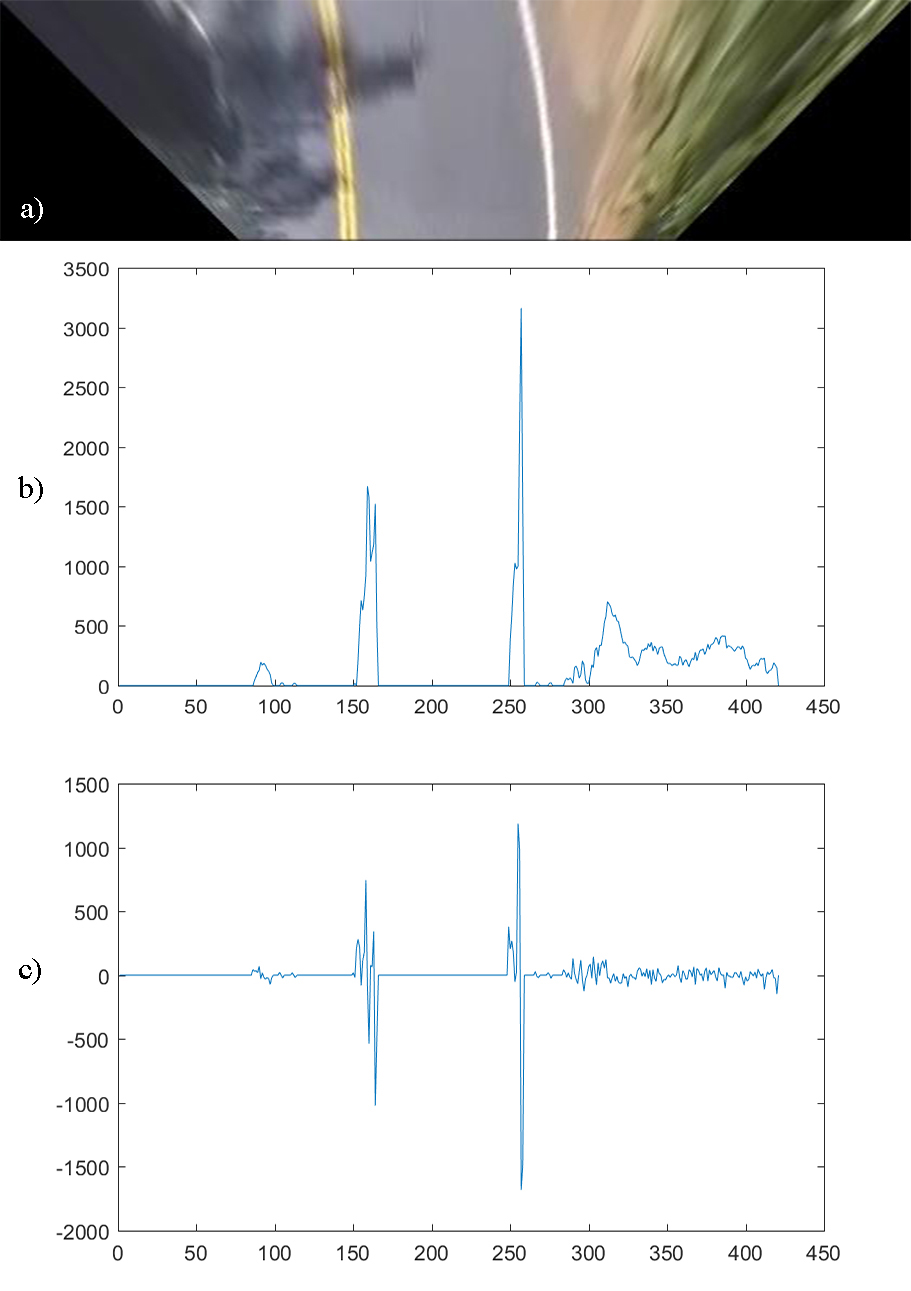
\includegraphics[max width=15cm,max height=15cm,keepaspectratio]{img_3_5}
	\caption[Linii din semnal]{a) Imaginea IPM b) Sumele cumulate ale imagini IPM filtrată pe coloane c) Normalizarea semnalului prin aplicarea filtrului Gaussian.}
\end{figure}

\subsubsection*{Etapa 5: Determinare linii finale}

Această ultimă etapă este împărțite în alte etape după cum urmează \hyperlink{WaymoSystem}{[11]}.

\textbf{A. Generează random puncte}
Această funcție are rolul de a genera un număr prestabilit de puncte din zona celor două maxime găsite la pasul anterior. În aplicația noastră acest număr a fost setat la 10.

\textbf{B. Potrivire puncte generate}
Pentru cele $n$ puncte generate, în cazul nostru 10, asignăm o valoare $t_i \in [0, 1]$ pentru fiecare punct $p_i = (u_i, v_i)$. Definim
\begin{align}
	t_i = \frac{\sum_{j = 1}^{i} d(p_j,p_{j-1})}{\sum_{j = 1}^{n} d(p_j,p_{j-1})} \quad pentru \quad t_i = 1, ..., n
\end{align}
$d$ reprezintă distanța euclidiană dată de formula
\begin{align}
	d(p_i,p_j) = \sqrt{(u_i - u_j)^2 + (v_i - v_j)^2}
\end{align}

În continuare, folosim datele obținute pentru a crea următoarele matrice.
\begin{center}
	$ Q = 
	\begin{bmatrix}
	p_1 \\
	... \\
	p_n \\
	\end{bmatrix}
	$ și $ T = 
	\begin{bmatrix}
	t_1^3 & t_1^2 & t_1 & 1 \\
	...\\
	t_n^3 & t_n^2 & t_n & 1\\
	\end{bmatrix}
	$
\end{center}

În final obținem punctele după următoarea formulă
\begin{align}
	P = (TM)^+Q
\end{align}
unde $(TM)^+$ reprezintă pseudoinversa matricei $TM$.

\textbf{C. Determină scorul asociat noilor puncte}
În final, calculăm pentru fiecare linie generată de punctele procesate un scor ce se bazează pe penalizarea liniilor scurte și/sau foarte curbate. Scor-ul este obținut pe baza formulei:
\begin{align}
	scor = s(1 + k_1l^{'}+k_2\theta^{'})
\end{align}
unde

$s$ - reprezintă suma pixelilor determinată de linia punctelor;

$l^{'} = (l/v) - 1$ - unde $l$ este lungimea liniei, $v$ este înalțimea imaginii, astfel dacă $l^{'}$ este 0 atunci aveam o linie foarte lungă, iar daca este -1 aveam o linie foarte scurtă;

$\theta^{'} = (\theta - 1)/2$ - unde $\theta = (cos\theta_1 + cos\theta_2)/2$;

$k_1$ și $k_2$ - sunt factori de regularizare prestabiliți, în cazul nostru $k_1 = k_2 = 0.5$.

În figura 3.6 sunt prezentate vizual componentele necesare determinării scorului.
\begin{figure}[!h]
	\centering
	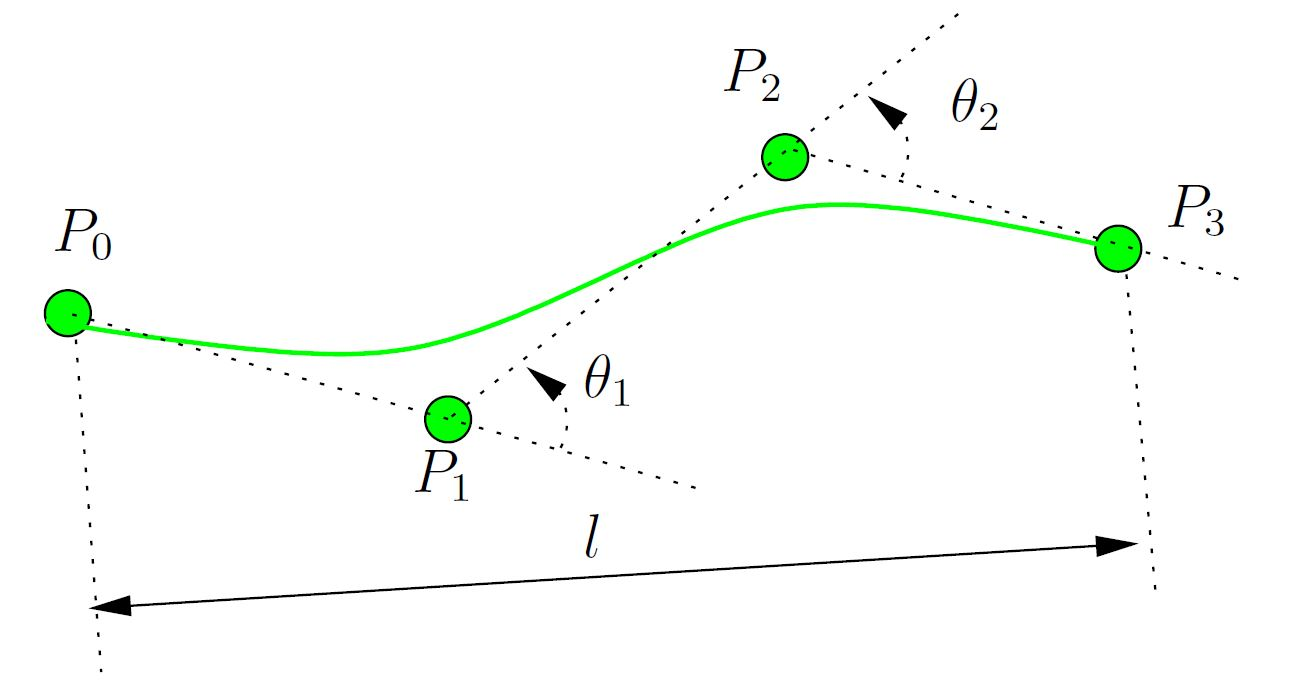
\includegraphics[max width=15cm,max height=15cm,keepaspectratio]{img_3_6}
	\caption[Determinare scor linie]{Determinare scor linie. Imagine preluată din \hyperlink{MohamedAly}{[11]}.}
\end{figure}

\textbf{D. Determinare cea mai bună linie}
În această ultimă etapă rulăm de un număr $N$ prestabilit de ori, în cazul nostru 30, pașii 1 - 3 și alegem din aceste $N$ rulări cel mai bun (mare) scor și implicit punctele asociate lui.

Aceste puncte rezultate sunt cele corespunzătoare imaginii IPM. Pentru a le aduce în planul imaginii de interes, imaginea de la care am plecat, avem nevoie de inversa matricei ce a dus punctele în planul IPM, inversă pe care o utilizăm cu funcția din OpenCV $cv.perspectiveTransform$. 

În acest punct, toate datele obținute sunt raportate la zona noastră de interes.

\section{Detectare mașină}
\subsection*{Noțiuni introductive}

A doua componentă esențială aplicației dezvoltate este cea reprezentată de detectarea de mașini. Aceasta primește de la prima componentă banda de circulație detectată, iar pe baza acesteia încearcă să găsească mașini strict în zona respectivă.

\subsection*{Algoritm detecție mașină}
Detecția mașinii, în situația de față, presupune două etape. Prima etapă preliminară este cea de antrenare a clasificatorilor, iar cea de-a doua este detectarea propriu-zisă a mașinii.

\textbf{Etapa I - Antrenarea clasificatorilor}

\textbf{Extragerea descriptorilor}

Primul pas în antrenarea clasificatorilor este reprezentat de extragerea descriptorilor din exemplele pozitive și negative. 
Acest lucru se va face cu funcția $vl\_hog$ din biblioteca $VLFeat$. 

\textbf{Antrenarea}

Toate exemplele negative vor forma un set de date. Cele patru clase de exemple pozitive vor fi antrenate separat cu setul de exemple negative. Astfel, vom obține patru vectori suport mașină pentru cele patru tipuri de imagini cu mașini. 
Pentru antrenare se va folosi funcția $vl\_svmtrain$ din biblioteca $VLFeat$.

\textbf{Etapa II - Detectarea propriu-zisă}

\textbf{Extragere regiune interes}

După cum a fost menționat anterior la detecția benzii curente de circulație vom folosi în continuare aceste informații pentru a elimina zona redundantă căutării mașinii în imagine.

\textbf{Anticipare poziție mașină}

Pentru a mări și mai mult viteza de rulare a programului se poate reduce zona de interes în care este foarte probabil să se afle o mașină cu ajutorul filtrelor de muchii, spre exemplu filtru Sobel pentru muchii orizontale și verticale pe baza următoarelor formule

\begin{align}
	\frac{\partial I(x,y)}{\partial x}
	\quad \quad
	\frac{\partial I(x,y)}{\partial y}
\end{align}

Figura 3.7 ilustrează un exemplu în acest sens.
\begin{figure}[!h]
	\centering
	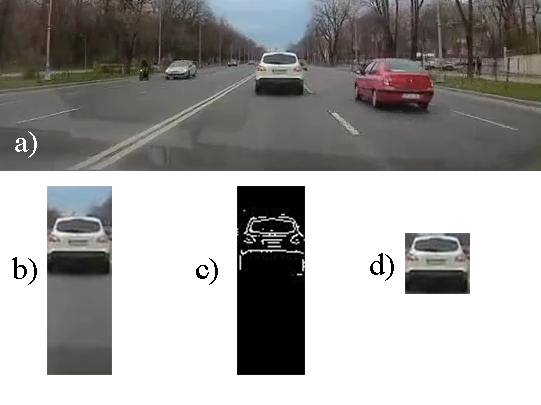
\includegraphics[max width=15cm,max height=15cm,keepaspectratio]{img_3_7}
	\caption[Regiune interes detecție mașină]{a) Imaginea inițială b) Imaginea rezultată pe baza detecției benzii c) Aplicarea filtrelor de muchii d) Extragerea zonei finale de interes.}
\end{figure}

\textbf{Rulare detector mașină}

Ultima fază din acest proces confirmă sau infirmă existența unei mașini în regiunea extrasă anterior. Pentru aceasta imaginea este mărită cu un factor de scală de 1.2 de 3 ori și micșorată cu un factor de scală 0.9 până când dimensiunea dimensiunea imaginii de analizat ajunge la $31 \times 31$ de pixeli, iar pe fiecare dintre aceaste 3 imagini, în cazul primului tip de operație executat asupra imaginii, plus cele n imagini, în cazul celui de-al doilea tip de operație executat asupra imaginii, se aplică metoda glisării ferestrei pentru a extrage caracteristici din imagine cu ajutorul HOG. În final, aceste caracteristici sunt trecute prin cele patru tipuri de mașini cu vectori suport, iar dacă cel puțin unul returnează un scor mai mare sau egal cu pragul stabilit de noi pentru respectiva porțiune, afirmăm că există o mașină pe banda curentă de circulație.

\section{Determinare distanță}
\subsection*{Noțiuni introductive}

O primă componentă secundară este cea care determină distanța până la eventuala mașină detectată pe banda curentă de circulație. Figura 3.8 prezintă un exemplu practic.

\subsection*{Algoritm determinare distanță}

Această componentă se folosește de detectarea de mașină prezentată anterior. Mai exact, aceasta trece în planul IPM coordonatele centrului detecției mașinii, iar din acel punct până la baza imaginii care reprezintă în IPM locația mașinii din care este realizat video-ul, se determină cu ajutorul raportării la o configurație 1 metru = n pixeli distanța efectivă în cadrul curent. Configurația este direct determinată de amplasarea camerei și tipul de video produs de aceasta. 

Pentru a evita schimbările foarte rapide de distanță, o detecție într-un frame nou este acceptată ca fiind o nouă detecție doar în situația în care diferența euclidiană dintre centrul detecției curente în planul IPM și centrul detecției anterioare în același plan depășește un anumit prag stabilit în prealabil.

\section{Determinare viteză relativă}
\subsection*{Noțiuni introductive}

O ultimă componentă, în prezenta aplicație, se ocupă de calcularea vitezei relative de deplasare a mașinii din față de pe banda curentă de circulație față de mașina din care este înregistrat video-ul, astfel existând trei situații de raspuns a acestei componente:

\begin{itemize}
	\item Viteza de deplasare a mașinii din față este mai mare;
	\item Viteza de deplasare a mașinii din față este similară;
	\item Viteza de deplasare a mașinii din față este mai mică;
\end{itemize}

Figura 3.8 prezintă un exemplu practic.
\begin{figure}[!h]
	\centering
	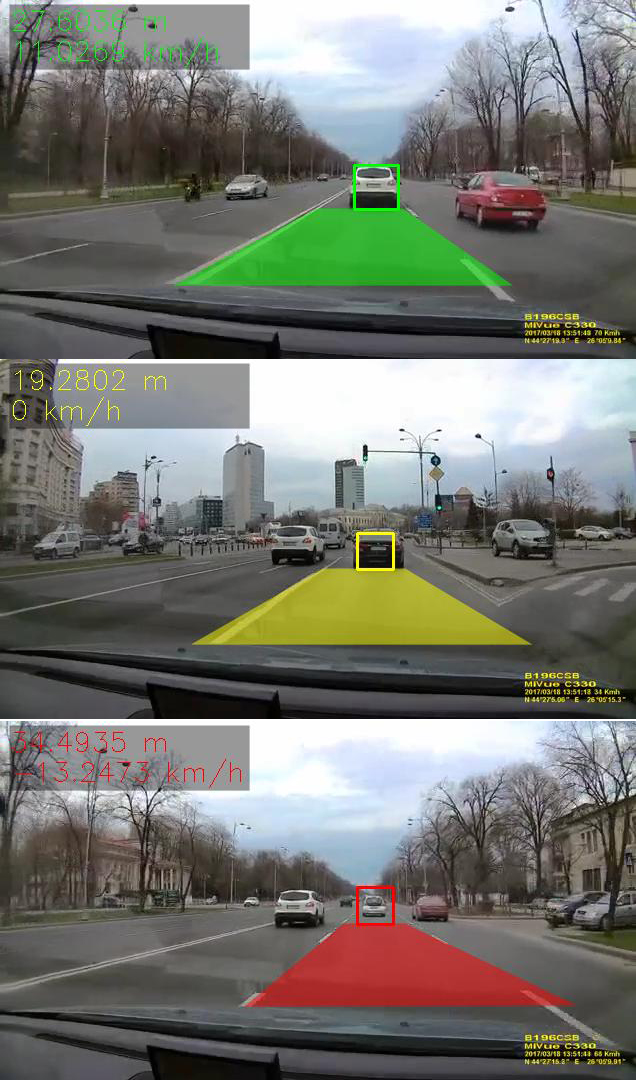
\includegraphics[max width=15cm,max height=15cm,keepaspectratio]{img_3_8}
	\caption[Determinare distanță și viteză]{a) Distanță 27 m, viteză relativă +11 km/h b) Distanță 19 m, viteză relativă +0 km/h c) Distanță 34 m, viteză relativă -13 km/h .}
\end{figure}

\subsection*{Algoritm determinare viteză relativă}

Precum componenta de detectare a distanței față de mașina din față și această componentă se folosește de detectarea de mașină prezentată anterior. Însă, de data aceasta se folosesc perechi de două frame-uri pentru a determina viteza relativă. Mai exact, aceasta trece în planul IPM coordonatele centrului detecției mașinii atât în frame-ul curent cât și în cel anterior, iar diferența dintre aceste două puncte o vom înmulți cu 3.6 pentru a obține kilometri pe oră. Configurația este direct determinată de amplasarea camerei și tipul de video produs de aceasta. 

Pentru a evita schimbările foarte rapide de viteză, o detecție într-un frame nou este acceptată ca fiind o nouă detecție doar în situația în care diferența euclidiană dintre centrul detecției curente în planul IPM și centrul detecției anterioare în același plan depășește un anumit prag stabilit în prealabil.